\section{Решение}

Я решил создать более общий вариант, кривая любого размера, с интерфейсом, возможностью добавления вершины в конец, удаление вершины из любого места массива точек, также изменение положения любой точки, также как и изменения направления опорных точек, по которым строится кривая.



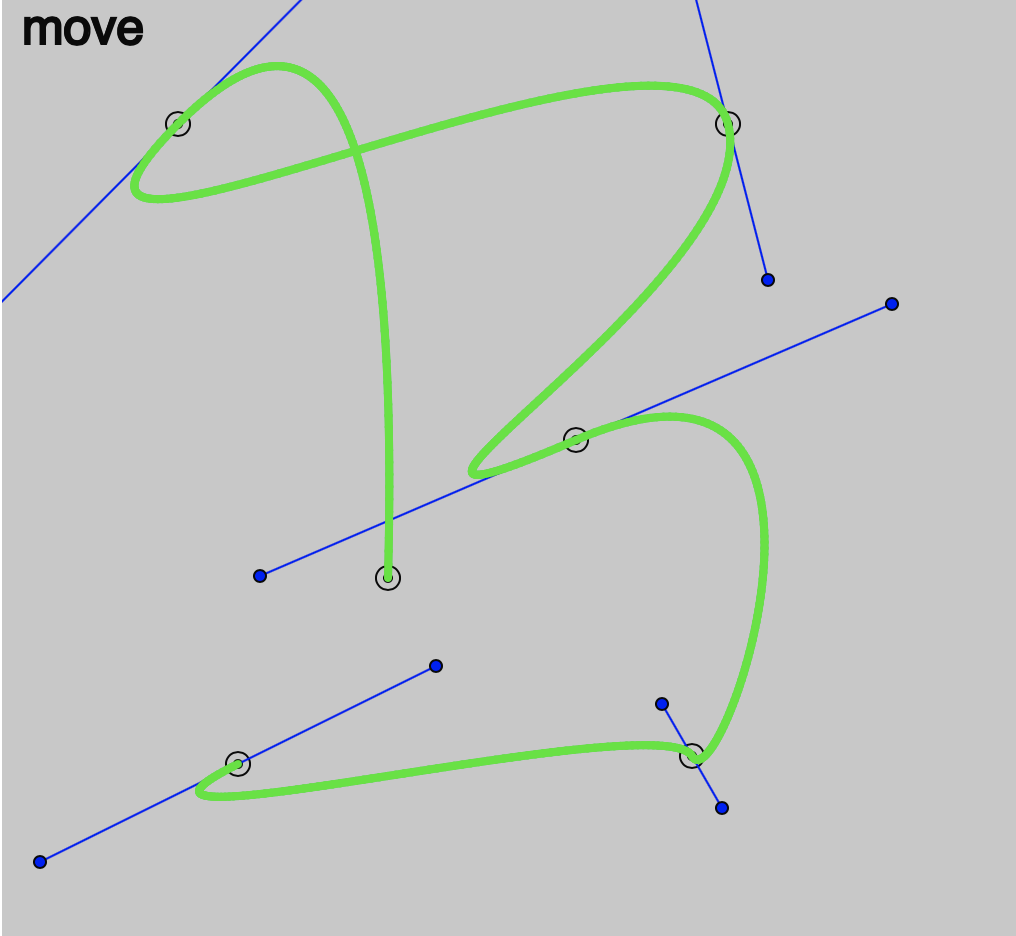
\includegraphics[scale=0.5]{pictures/1.png}

Кривая неограничена по размерам, длине, кол-во опорных точек у каждой вершины от нуля до двух, повторным нажатием в режиме draw позволяет менять положение опорных точек, отводя с зажатой мышью курсор от вершины. Интерфейс интуитивно понятен.

Алгоритм хранится в себе массив вершин, в которой хранятся координаты двух опорных точек. Далее в цикле для точки имеющей два соседа считаются промежуточные координаты кривой по 4 точкам, рекурсивно сводя до трех, а потом для двух точек. Что можно рассматривать как кубическую кривую Безье.

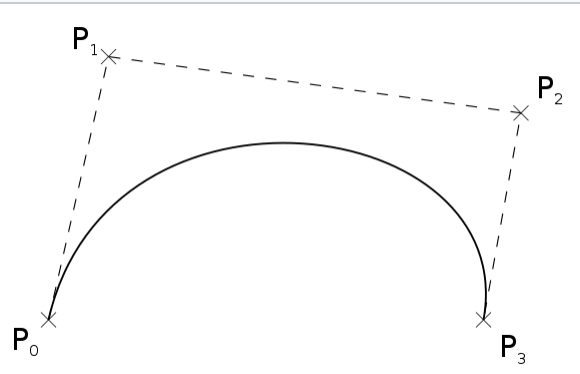
\includegraphics[scale=0.5]{pictures/3.png}

Если же у вершины существует только левый или правый сосед, Алгоритм начиает просчитывать кривую для трех вершин, сводя ее к двум. Что можно рассмаривать как квадратичную кривую Безье.

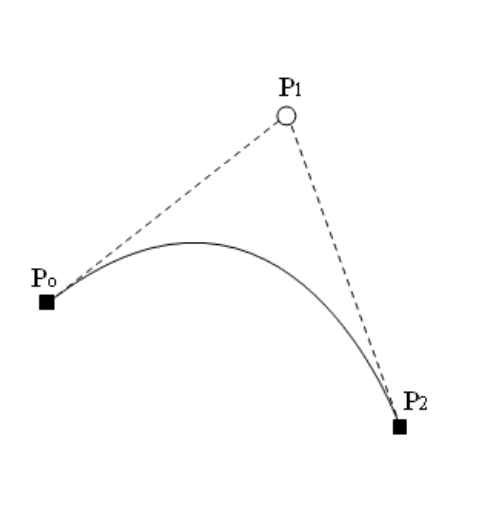
\includegraphics[scale=0.5]{pictures/2.png}

